\documentclass{standalone}
\usepackage{tikz}
\begin{document}
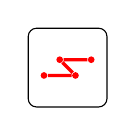
\begin{tikzpicture}[scale=1.0]
  % draw rounded cell boxes
  \draw[rounded corners=3pt] (0,0) rectangle (1,1);
  \node[circle, fill=red, inner sep=0.03cm] (obs4385736464_pt0) at (0.2,0.4) {};
  \node[circle, fill=red, inner sep=0.03cm] (obs4385736464_pt1) at (0.4,0.6000000000000001) {};
  \node[circle, fill=red, inner sep=0.03cm] (obs4385736464_pt2) at (0.6,0.4) {};
  \node[circle, fill=red, inner sep=0.03cm] (obs4385736464_pt3) at (0.8,0.6000000000000001) {};
  \draw[red, line width=1.2pt] (obs4385736464_pt0) -- (obs4385736464_pt2) -- (obs4385736464_pt1) -- (obs4385736464_pt3);
\end{tikzpicture}
\end{document}